% Rebuild (from repo root):
%   pdflatex -interaction=nonstopmode -output-directory=docs docs/where_the_ai_should_run.tex
%   pdflatex -interaction=nonstopmode -output-directory=docs docs/where_the_ai_should_run.tex
%   mv docs/where_the_ai_should_run.pdf docs/Where-the-AI-Should-Run-Companion-vs-Flight-Controller.pdf
\documentclass[11pt,a4paper]{article}

\usepackage[T1]{fontenc}
\usepackage[utf8]{inputenc}
\usepackage{libertine}
\usepackage[defaultsans,tabular,lining]{lato}
\renewcommand{\familydefault}{\sfdefault}

\usepackage[
  a4paper,
  top=22mm,
  bottom=20mm,
  left=24mm,
  right=24mm
]{geometry}
\usepackage{xcolor}
\usepackage{microtype}
\usepackage{parskip}
\usepackage{tikz}
\usetikzlibrary{arrows.meta,positioning,calc}

\pagestyle{empty}
\thispagestyle{empty}

\definecolor{navy}{HTML}{1B365D}
\definecolor{ink}{HTML}{1F2430}
\definecolor{body}{HTML}{2A3140}
\definecolor{quiet}{HTML}{5A6270}
\definecolor{mute}{HTML}{8A93A0}
\definecolor{line}{HTML}{C5CCD6}
\definecolor{cardline}{HTML}{D5DBE3}
\definecolor{wash}{HTML}{F4F7FB}
\definecolor{optbody}{HTML}{3A414C}

\color{ink}
\setlength{\parskip}{0pt}
\setlength{\parindent}{0pt}

\newcommand{\seriftitle}{\rmfamily\bfseries\color{navy}}
\newcommand{\sectionline}[1]{%
  {\seriftitle\fontsize{14}{18}\selectfont #1}\par\vspace{3.2mm}%
}

\begin{document}

{\seriftitle\fontsize{26}{30}\selectfont Where should the AI run?\par}
\vspace{8mm}

{\fontsize{12}{17}\selectfont\color{body}%
Sir asked: can we apply this research on the flight controller, or through Mission Planner? Which is easier?\par}
\vspace{5.5mm}

{\seriftitle\fontsize{13.5}{18}\selectfont
Neither. The easy and correct place is a companion computer with PX4.\par}
\vspace{2.6mm}

{\fontsize{11}{16}\selectfont\color{body}%
The flight controller only flies the drone. Mission Planner is ground software for a different autopilot. Our AI needs a small Linux board on the drone.\par}
\vspace{6mm}

{\fontsize{9.5}{14}\selectfont\color{quiet}%
A \textbf{\color{navy}flight controller} (Pixhawk) is the tiny chip that keeps the drone in the air. A \textbf{\color{navy}companion computer} is an extra Linux board for heavier work such as cameras and neural nets. \textbf{\color{navy}Mission Planner} is laptop software, mainly for ArduPilot. This project already uses \textbf{\color{navy}PX4}.\par}
\vspace{7mm}

\noindent
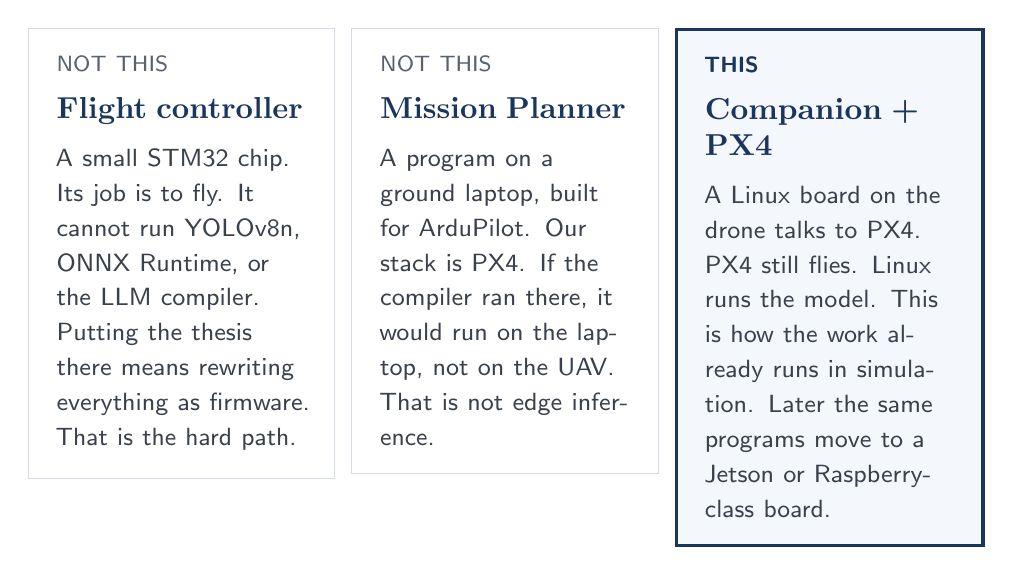
\begin{tikzpicture}[x=\linewidth]
  \def\gap{0.018}
  \def\w{0.321}
  \node[anchor=north west, inner sep=3.6mm, text width=0.321\linewidth-7.2mm,
        draw=cardline, line width=0.4pt, fill=white, minimum height=41mm]
        (a) at (0,0) {
    {\fontsize{8}{10}\selectfont\color{quiet}\MakeUppercase{Not this}\par}
    \vspace{1.4mm}
    {\seriftitle\fontsize{11}{13}\selectfont Flight controller\par}
    \vspace{1.6mm}
    {\fontsize{9}{12.6}\selectfont\color{optbody}A small STM32 chip. Its job is to fly. It cannot run YOLOv8n, ONNX Runtime, or the LLM compiler. Putting the thesis there means rewriting everything as firmware. That is the hard path.\par}
  };
  \node[anchor=north west, inner sep=3.6mm, text width=0.321\linewidth-7.2mm,
        draw=cardline, line width=0.4pt, fill=white, minimum height=41mm]
        (b) at ({\w+\gap},0) {
    {\fontsize{8}{10}\selectfont\color{quiet}\MakeUppercase{Not this}\par}
    \vspace{1.4mm}
    {\seriftitle\fontsize{11}{13}\selectfont Mission Planner\par}
    \vspace{1.6mm}
    {\fontsize{9}{12.6}\selectfont\color{optbody}A program on a ground laptop, built for ArduPilot. Our stack is PX4. If the compiler ran there, it would run on the laptop, not on the UAV. That is not edge inference.\par}
  };
  \node[anchor=north west, inner sep=3.6mm, text width=0.321\linewidth-7.2mm,
        draw=navy, line width=1.1pt, fill=wash, minimum height=41mm]
        (c) at ({2*(\w+\gap)},0) {
    {\fontsize{8}{10}\selectfont\color{navy}\textbf{\MakeUppercase{This}}\par}
    \vspace{1.4mm}
    {\seriftitle\fontsize{11}{13}\selectfont Companion + PX4\par}
    \vspace{1.6mm}
    {\fontsize{9}{12.6}\selectfont\color{optbody}A Linux board on the drone talks to PX4. PX4 still flies. Linux runs the model. This is how the work already runs in simulation. Later the same programs move to a Jetson or Raspberry-class board.\par}
  };
\end{tikzpicture}

\vspace{7mm}

\noindent
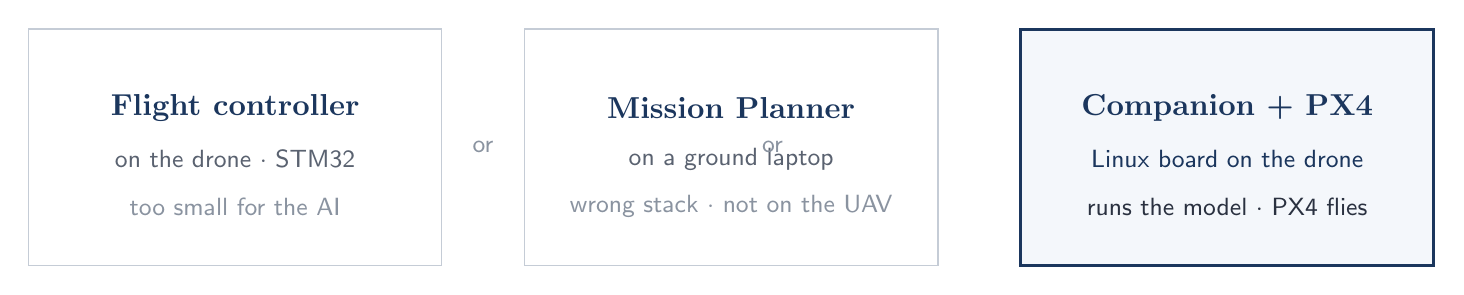
\begin{tikzpicture}[x=1mm, y=1mm]
  \def\boxw{52.5}
  \def\boxh{30}
  \def\gapx{10.5}
  \coordinate (p1) at (0,0);
  \coordinate (p2) at ({\boxw+\gapx},0);
  \coordinate (p3) at ({2*(\boxw+\gapx)},0);

  \draw[line width=0.5pt, color=line] (p1) rectangle ++(\boxw,\boxh);
  \node[font=\rmfamily\bfseries\color{navy}\fontsize{11}{13}\selectfont] at ($(p1)+(0.5*\boxw,20)$) {Flight controller};
  \node[font=\color{quiet}\fontsize{9}{11}\selectfont] at ($(p1)+(0.5*\boxw,13.5)$) {on the drone $\cdot$ STM32};
  \node[font=\color{mute}\fontsize{9}{11}\selectfont] at ($(p1)+(0.5*\boxw,7.5)$) {too small for the AI};

  \node[font=\color{mute}\fontsize{9}{11}\selectfont] at ({(\boxw+\gapx/2)},15) {or};

  \draw[line width=0.5pt, color=line] (p2) rectangle ++(\boxw,\boxh);
  \node[font=\rmfamily\bfseries\color{navy}\fontsize{11}{13}\selectfont] at ($(p2)+(0.5*\boxw,20)$) {Mission Planner};
  \node[font=\color{quiet}\fontsize{9}{11}\selectfont] at ($(p2)+(0.5*\boxw,13.5)$) {on a ground laptop};
  \node[font=\color{mute}\fontsize{9}{11}\selectfont] at ($(p2)+(0.5*\boxw,7.5)$) {wrong stack $\cdot$ not on the UAV};

  \node[font=\color{mute}\fontsize{9}{11}\selectfont] at ({(1.5*\boxw+1.5*\gapx)},15) {or};

  \fill[wash] (p3) rectangle ++(\boxw,\boxh);
  \draw[line width=1.1pt, color=navy] (p3) rectangle ++(\boxw,\boxh);
  \node[font=\rmfamily\bfseries\color{navy}\fontsize{11}{13}\selectfont] at ($(p3)+(0.5*\boxw,20)$) {Companion + PX4};
  \node[font=\color{navy}\fontsize{9}{11}\selectfont] at ($(p3)+(0.5*\boxw,13.5)$) {Linux board on the drone};
  \node[font=\color{body}\fontsize{9}{11}\selectfont] at ($(p3)+(0.5*\boxw,7.5)$) {runs the model $\cdot$ PX4 flies};
\end{tikzpicture}

\vspace{2mm}
{\fontsize{9}{13}\selectfont\color{quiet}%
Three places people might put the AI. Only the companion computer on the drone is both possible and on the UAV.\par}

\newpage
\thispagestyle{empty}

\sectionline{How the work is split}

{\fontsize{11}{16}\selectfont\color{ink}%
Atul's notes put it simply: the flight controller is not strong enough for video or AI, so the drone needs a second computer. The LLM only thinks about compile choices. It does not fly the drone.\par}
\vspace{6mm}

\noindent
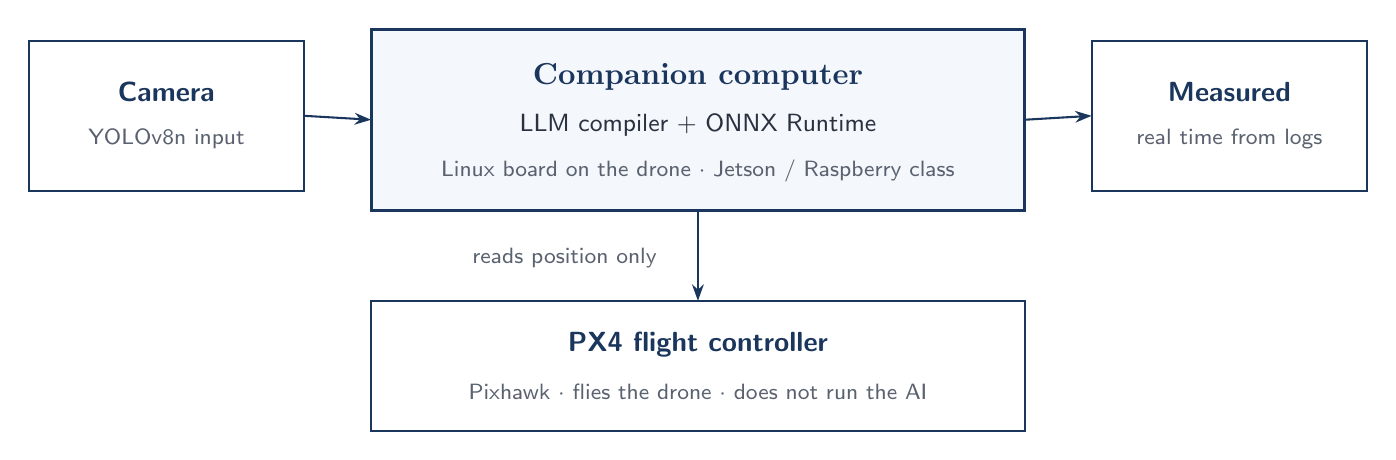
\begin{tikzpicture}[x=1mm, y=1mm, >= {Stealth[length=2.1mm, width=1.5mm]}]
  \def\cw{83}
  \def\ch{23}
  \def\sw{35}
  \def\sh{19}
  \coordinate (comp) at (43.5,28);
  \coordinate (cam) at (0,30.5);
  \coordinate (meas) at (135,30.5);
  \coordinate (fc) at (43.5,0);

  \draw[line width=0.7pt, color=navy] (cam) rectangle ++(\sw,\sh);
  \node[font=\bfseries\color{navy}\fontsize{10}{12}\selectfont] at ($(cam)+(0.5*\sw,12.5)$) {Camera};
  \node[font=\color{quiet}\fontsize{8.5}{10}\selectfont] at ($(cam)+(0.5*\sw,6.5)$) {YOLOv8n input};

  \fill[wash] (comp) rectangle ++(\cw,\ch);
  \draw[line width=1.1pt, color=navy] (comp) rectangle ++(\cw,\ch);
  \node[font=\rmfamily\bfseries\color{navy}\fontsize{11}{13}\selectfont] at ($(comp)+(0.5*\cw,17)$) {Companion computer};
  \node[font=\color{body}\fontsize{9}{11}\selectfont] at ($(comp)+(0.5*\cw,10.8)$) {LLM compiler + ONNX Runtime};
  \node[font=\color{quiet}\fontsize{8}{10}\selectfont] at ($(comp)+(0.5*\cw,5)$) {Linux board on the drone $\cdot$ Jetson / Raspberry class};

  \draw[line width=0.7pt, color=navy] (meas) rectangle ++(\sw,\sh);
  \node[font=\bfseries\color{navy}\fontsize{10}{12}\selectfont] at ($(meas)+(0.5*\sw,12.5)$) {Measured};
  \node[font=\color{quiet}\fontsize{8.5}{10}\selectfont] at ($(meas)+(0.5*\sw,6.5)$) {real time from logs};

  \draw[line width=0.7pt, color=navy] (fc) rectangle ++(\cw,16.5);
  \node[font=\bfseries\color{navy}\fontsize{10}{12}\selectfont] at ($(fc)+(0.5*\cw,11)$) {PX4 flight controller};
  \node[font=\color{quiet}\fontsize{8.5}{10}\selectfont] at ($(fc)+(0.5*\cw,5)$) {Pixhawk $\cdot$ flies the drone $\cdot$ does not run the AI};

  \draw[navy, line width=0.75pt, ->] ($(cam)+(\sw,0.5*\sh)$) -- ($(comp)+(0,0.5*\ch)$);
  \draw[navy, line width=0.75pt, ->] ($(comp)+(\cw,0.5*\ch)$) -- ($(meas)+(0,0.5*\sh)$);
  \draw[navy, line width=0.75pt, ->] ($(comp)+(0.5*\cw,0)$) -- ($(fc)+(0.5*\cw,16.5)$);
  \node[font=\color{quiet}\fontsize{8}{10}\selectfont, anchor=east] at ($(comp)+(0.5*\cw-4,-6)$) {reads position only};
\end{tikzpicture}

\vspace{2mm}
{\fontsize{9}{13}\selectfont\color{quiet}%
Same split as the notebook: camera and neural net on the companion; Pixhawk only flies. Groq may suggest compile strategies. It is not the measured run. If a ground screen is needed later, use QGroundControl to watch PX4 --- do not put the compiler there.\par}

\vspace{8mm}
\sectionline{Today, and later}

\noindent

\begin{tikzpicture}[x=1mm, y=1mm, >= {Stealth[length=2.1mm, width=1.5mm]}]
  \def\bw{71.5}
  \def\bh{23}
  \coordinate (today) at (0,0);
  \coordinate (later) at (105.5,0);

  \draw[line width=0.7pt, color=navy] (today) rectangle ++(\bw,\bh);
  \node[font=\color{mute}\fontsize{8}{10}\selectfont] at ($(today)+(0.5*\bw,17.5)$) {Today $\cdot$ simulation};
  \node[font=\rmfamily\bfseries\color{navy}\fontsize{11}{13}\selectfont] at ($(today)+(0.5*\bw,11)$) {Linux PC + PX4 SITL};
  \node[font=\color{quiet}\fontsize{8.5}{10}\selectfont] at ($(today)+(0.5*\bw,4.8)$) {same idea, simulated drone};

  \draw[navy, line width=0.75pt, ->] ($(today)+(\bw,0.5*\bh)$) -- ($(later)+(0,0.5*\bh)$);
  \node[font=\color{navy}\fontsize{8}{10}\selectfont] at (88.5,16.5) {same programs};

  \fill[wash] (later) rectangle ++(\bw,\bh);
  \draw[line width=1.1pt, color=navy] (later) rectangle ++(\bw,\bh);
  \node[font=\color{navy}\fontsize{8}{10}\selectfont] at ($(later)+(0.5*\bw,17.5)$) {Later $\cdot$ real airframe};
  \node[font=\rmfamily\bfseries\color{navy}\fontsize{11}{13}\selectfont] at ($(later)+(0.5*\bw,11)$) {Companion + Pixhawk};
  \node[font=\color{body}\fontsize{8.5}{10}\selectfont] at ($(later)+(0.5*\bw,4.8)$) {Linux board runs AI $\cdot$ Pixhawk flies};
\end{tikzpicture}

\vspace{2mm}
{\fontsize{9}{13}\selectfont\color{quiet}%
Already working in simulation: ONNX compiler, YOLOv8n, ROS inference on the Linux host, PX4 SITL with live position. TensorRT is skipped here because this machine has no NVIDIA GPU.\par}

\vspace{9mm}
\sectionline{For the thesis}

{\fontsize{11}{16}\selectfont\color{ink}%
We continue with companion + PX4. We will not put the compiler inside flight-controller firmware. We will not build a Mission Planner plugin.\par}
\vspace{2.4mm}
{\fontsize{11}{16}\selectfont\color{ink}%
The LLM may only suggest allowed compile strategies. The compiler checks and compiles. The profiler measures real time from logs. Telemetry only reads position. The AI does not take over flying.\par}

\end{document}
